\documentclass[a4paper,12pt]{article} 
\usepackage{baseset}
\DeclareSymbolFont{operators}{OT1}{ntxtlf}{m}{n}
\SetSymbolFont{operators}{bold}{OT1}{ntxtlf}{b}{n}
\usepackage{wasysym}
\usepackage{multirow}
\graphicspath{{images/}}
\DeclareGraphicsExtensions{.pdf,.png,.jpg}

%Заговолок
\author{Красоткина Виктория}

\title{Лабораторная работа 1.4.8

Измерение модуя Юнга методом аккустического резонанса}

\date{14 ноября 2022 г.}

\begin{document}

\maketitle
\thispagestyle{empty}

\newpage
\setcounter{page}{1}

\textbf{Цель:}
Определить скорость полета пули, применяя законы сохранения и используя баллистические маятники.

\textbf{Приборы:}
\begin{itemize}
    \item духовое ружье на штативе
    \item осветитель
    \item оптическая система для измерения отклонений маятника
    \item измерительная линейка
    \item пули и весы для их взвешивания
    \item пинцет
    \item также баллистические маятники
\end{itemize}

\subsection*{Теоретическая часть}   
	Относительная деформация по оси, вдоль которой приложено механическое напряжение $\sigma$:  $\varepsilon = \dfrac{\Delta x}{x_0}$ определяется соотношением:
	$$
	\sigma=\varepsilon E
	$$

	Скорость $u$ распространения продольной акустической волны, вызванной малой деформацией тела, в случае длинного тонкого стержня определяется соотношением:
	$$
	u=\sqrt{\frac{E}{\rho}}
	$$

	С точки зрения распространения волн стержень
	можно считать тонким, если длина $\lambda$ звуковых волн в нём велика по сравнению с его радиусом: $\lambda \ll R$. Такая волна свободно распространяется только вдоль стержня, поэтому можно считать, что стержень испытывает деформации растяжения и сжатия только вдоль своей оси.

	Если боковые стенки тонкого
	стержня свободны, то его деформации описывается законом Гука, и, упругие свойства
	определяются модулем Юнга среды.
	
	Акустическая волна, распространяющаяся в стержне конечной длины $L$,
	испытает отражение от торцов стержня. Если при этом на длине стержня
	укладывается целое число полуволн, то отражённые волны будут складываться в фазе с падающими, что приведёт к резкому усилению амплитуды
	их колебаний и возникновению акустического резонанса в стержне. Измеряя соответствующие резонансные частоты, можно определить скорость
	звуковой волны в стержне и, таким образом, измерить модуль Юнга материала стержня.
	
	
	\subsubsection*{Уравнение волны в тонком стержне} 
	
	Направим ось $Ox$ вдоль геометрической оси стержня (рис. \ref{Sily}). Разобьём исходно недеформированный стержень на тонкие слои толщиной $\Delta x$. При продольной деформации среды границы слоёв сместятся в некоторые новые положения. Пусть плоскость среды, находящаяся исходно в точке $x$,
	сместилась к моменту $t$ на расстояние $\xi(x, t)$ Тогда слой, занимавший исходно отрезок $[x ; x+\Delta x]$, изменил свой продольный размер на величину $\Delta \xi=\xi(x+\Delta x, t)-\xi(x, t)$. Пользуясь малостью $\Delta x$ и определением производной, получим $\Delta \xi=\dfrac{\partial \xi}{\partial x} \Delta x$. Относительное удлинение элемента стержня в точке $x$.
	
	\begin{figure}[h!]
		\centering
		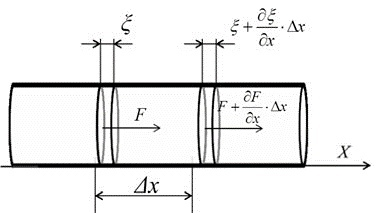
\includegraphics[scale=0.7]{1}
		\caption{Силы, действующие на элемент стержня при продольных колебаниях}
		\label{pic1}
	\end{figure}
	
	$$
	\Delta \xi=\frac{\partial \xi}{\partial x} \Delta x
	$$
	
	По закону Гука:
	$$
	\sigma=\varepsilon E=E \frac{\partial \xi}{\partial x},
	$$
	$\sigma = \dfrac{F}{S}$ ($F$ -- сила, $S$ -- площадь поперечного сечения.)
	
	Из-за разницы напряжений возникнет возвращающая сила:
	$$
	\Delta F=S \sigma(x+\Delta x)-S \sigma(x)=\frac{\partial \sigma}{\partial x} S \Delta x=\frac{\partial^{2} \xi}{\partial x^{2}} E S \Delta x
	$$
	Ускорение маленького элемента массой $\Delta m$:
	$$
	a=\frac{\partial^{2} \xi}{\partial t^{2}}
	$$
	Из предыдущих соотношений получаем уравнение движени среды:
	$$
	\operatorname{S\rho} \Delta x \frac{\partial^{2} \xi}{\partial t^{2}}=\operatorname{SE} \Delta x \frac{\partial^{2} \xi}{\partial x^{2}}
	$$
	Если принять $u = \sqrt{\dfrac{E}{p}}$ (скорость распространения волны в срерде) получаем волновое уравение:
	\begin{equation} 
		\label{dif}
		\operatorname{S\rho} \Delta x \frac{\partial^{2} \xi}{\partial t^{2}}=\operatorname{SE} \Delta x \frac{\partial^{2} \xi}{\partial x^{2}}
	\end{equation}
	
	\subsubsection*{Бегущие акустические волны. Скорость волны.}
	Решение волнового уравнения, зависящее от $X=x-u t$ - $\xi(x, t)=\phi(x-u t)$. Волновое уравнение обращается в тождество при любой $\phi(x-u t)$
	$$
	\frac{\partial^{2} \phi}{\partial t^{2}}=(-u)^{2} \phi^{\prime \prime}, \quad \frac{\partial^{2} \phi}{\partial x^{2}}=\phi^{\prime \prime} \rightarrow \frac{\partial^{2} \phi}{\partial t^{2}} \equiv u^{2} \frac{\partial^{2} \phi}{\partial x^{2}}
	$$
	$\phi(x-u t)$ описывает	возмущение среды произвольной формы, которое смещается поступательно во времени по оси $Ox$ со скоростью $u = \dfrac{d x}{d t}$, не меняя своей формы.
	
	Общее решение дифференциального уравнения \ref{dif} представимо в виде суммы двух волн произвольной формы, бегущих в противоположные стороны со скоростями $\pm u$:
	$$
	\xi(x, t)=\phi_{1}(x-u t)+\phi_{2}(x+u t),
	$$
	где $u$ — скорость волны, $\phi_1$ и $\phi_2$ — функции, вид которых в конкретной задаче определяется из начальных и граничных условий.
	
	\subsubsection*{Собственные колебания стержня}
	В случае гармонического возбуждения колебаний с частотой $f$ продольная волна в тонком стержне может быть представлена в виде суперпозиции двух бегущих навстречу гармонических волн:
	\begin{equation} 
		\label{garm}
		\xi(x, t)=A_{1} \sin \left(\omega t-k x+\varphi_{1}\right)+A_{2} \sin \left(\omega t+k x+\varphi_{2}\right),
	\end{equation}
	где $\omega = 2 \pi f$ — циклическая частота. Коэффициент $k = \dfrac{2 \pi}{\lambda}$ называют волновым числом или пространственной частотой волны. 
	
	Первое слагаемое \ref{garm} описывает гармоническую (синусоидальную) волну, бегущую в положительном направлении по $x$, второе -- в отрицательном. Соотношения между амплитудами $A_1, A_2$ и начальными фазами $\phi_1, \phi_2$ этих волн, а также возможные частоты колебаний $\omega$, определяются граничными условиями на концах стержня. 
	
	Пусть концы стержня не закреплены. Тогда напряжения в них должны равняться нулю. Пусть координаты торцов $x$ = 0 и $L$ = $x$. Получаем граничные условия для свободных концов стержня:
	$$
	\sigma(0)=\left.0 \rightarrow \frac{\partial \xi}{\partial x}\right|_{x=0}=0, \quad \sigma(L)=\left.0 \rightarrow \frac{\partial \xi}{\partial x}\right|_{x=L}=0
	$$
	Эти соотношения должны выполняться в произвольный момент времени. Получаем:
	$$
	-k A_{1} \cos \left(\omega t+\varphi_{1}\right)+k A_{2} \cos \left(\omega t+\varphi_{2}\right)=0
	$$
	Выполняется при любом $t$, если у падающией и отражённой волн равны:
	$$
	A_{1}=A_{2}
	$$
	$$
	\varphi_{1}=\varphi_{2}
	$$
	Амплитуды бедут равны, если волны отражаются без потери энергии. Равенство фаз означает то, что при отражении синусоидальной волны от свободного окнца стержня фаза не меняется. Перепишем исследуемую функцию \ref{dif}:
	$$
	\xi(x, t)=2 A \cos (k x) \sin (\omega t+\varphi)
	$$
	Такие колебания -- стоячие волны. 

	Выражая через длину волны получаем:
	$$
	\lambda_{n}=\frac{2 L}{n}, \quad n \in \mathbb{N}
	$$
	Для возбуждения стоячей волны на длине стрежня должно укладываться целое число полуволн.
	
	Допустимые значения частот -- собственные частоты колебаний стержня длиной $L$:
	$$
	f_{n}=\frac{u}{\lambda_{n}}=n \frac{u}{2 L}, \quad n \in \mathbb{N},
	$$
	При совпадении внешней частоты с одной из собственных частот в стежне возникает акустический резонанс.
	
	Зависимость амплитуды смещения $\xi$ от координаты $x$ для собственных колебаний стержня с незакреплёнными концами. Она распределена по гармоническому закону: $\xi_{0}(x)=2 A \cos k x$. В реальной системе стоячая волна не может	быть получена в чистом виде, так как всегда существуют потери энергии.
	
	\begin{figure}[h!] 
		\centering
		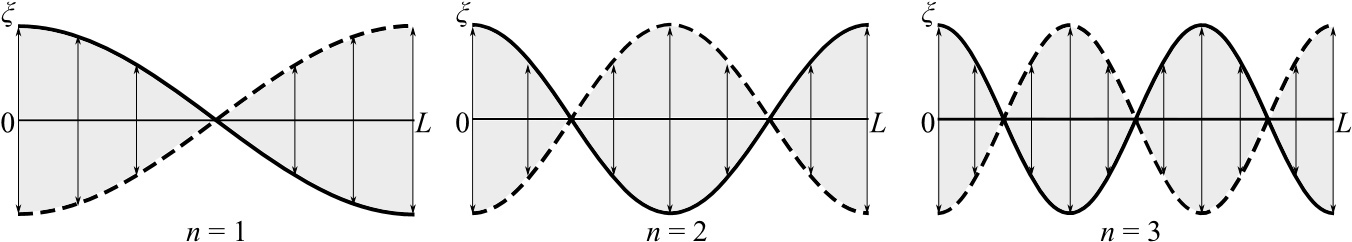
\includegraphics[scale=0.33]{2}
		\caption{Собственные продольные колебания стержня с незакреплёнными концами}
		\label{pic2}
	\end{figure}
	
	\subsubsection*{Схема и методика измерений}
	\begin{figure}[h]
		\centering
		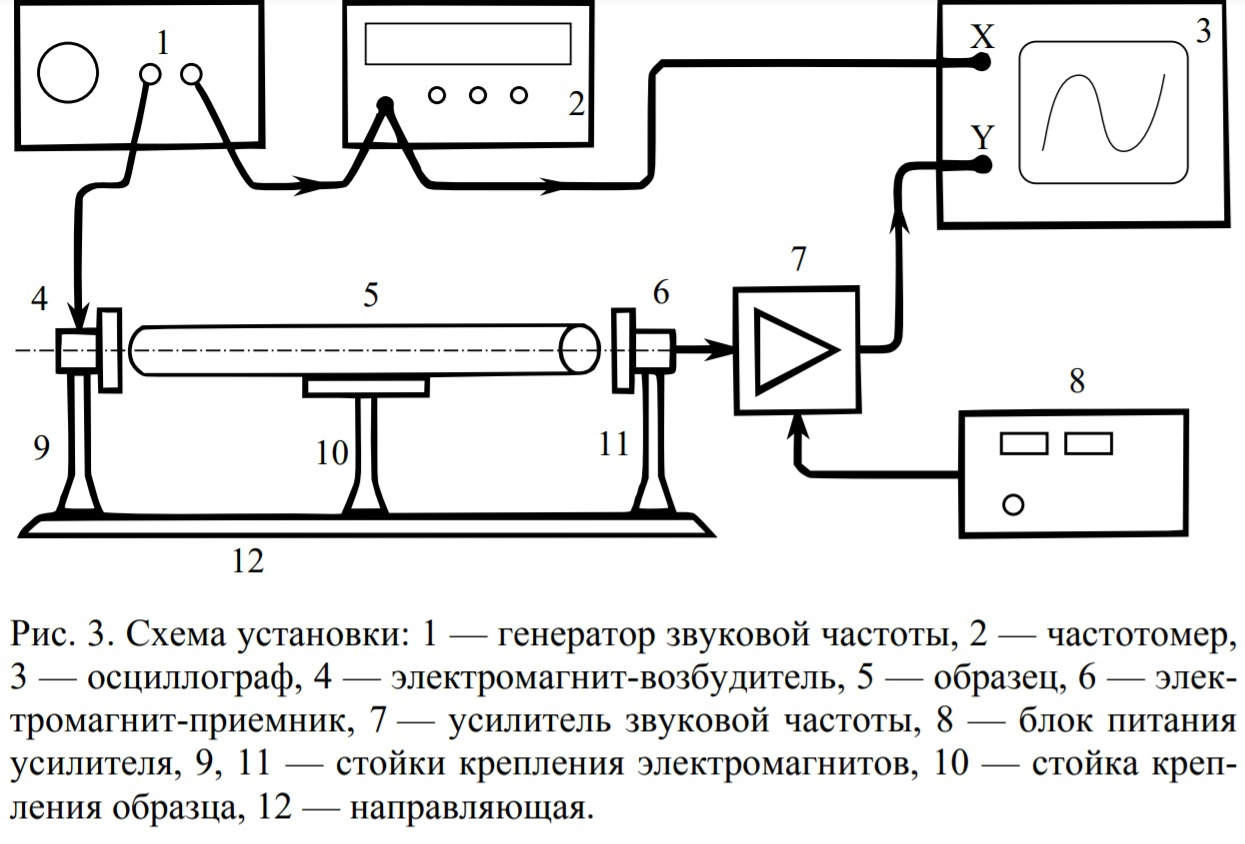
\includegraphics[scale=0.31]{3}
		\caption{Схема установки}
		\label{pic3}
	\end{figure}
	
	Исследуемый	стержень 5 размещается на стойке 10. Возбуждение и приём колебаний в стержне осуществляются электромагнитными преобразователями 4 и 6, расположенными рядом с торцами стержня. Крепления 9, 11 электромагнитов дают возможность регулировать их расположение по высоте, а также перемещать вправо-влево по столу 12. Электромагнит 4 служит для возбуждения упругих механических продольных колебаний в стержне. На него с генератора звуковой частоты 1 подаётся сигнал синусоидальной формы: протекающий в катушке электромагнита ток создаёт пропорциональное ему магнитное поле, вызывающее	периодическое воздействие заданной частоты на торец стержня. Рядом с другим торцом стержня находится аналогичный электромагнитный датчик 6, который служит для преобразования механических колебаний в электрические. Сигнал с выхода генератора поступает на частотомер 2 и на вход канала X осциллографа 3. ЭДС, возбуждаемая в регистрирующем электромагните 6, пропорциональная амплитуде колебаний торца стержня, усиливается усилителем 7 и подаётся на вход канала Y осциллографа. Изменяя частоту генератора и наблюдая за амплитудой сигнала с регистрирующего датчика, можно определить частоту акустического резонанса в стержне. Наблюдения в режиме X–Y позволяют сравнить сигналы генератора и датчика, а также облегчает поиск резонанса при слабом сигнале.
	
	\subsubsection*{Методика измерений}
	Модуль Юнга материала $E$ может быть найден по скорости распространения акустических волн в стержне $u$ и его плотности $\rho$. Для определения скорости используем метод аккустического резонанса. 
	
	Зная номер гармоники $n$ и резонансную частоту $\nu_n$, на которой наблюдается усиление амплитуды колебаний, вычисляем скорость распространения подольных волн в стержне:
	$$
	u=2 L \frac{f_{n}}{n}
	$$
	Таким образом, для измерения скорости $u$ необходимо измерить длину	стержня $L$ и получить зависимость резонансной частоты от номера резонанса $f_n(n)$. Принимаем во внимание только резонансы, опысываемые выше.
	
	\subsection*{Ход работы}
	Сперва определим погрешности приборов:
	\begin{itemize}
		\item штангенциркуль: $2\cdot\dfrac{\text{цена деления}}{2} = 0.1$ мм
		\item микрометр: $2\cdot\dfrac{\text{цена деления}}{2} = 1$ мкм
	\end{itemize}
	Систематическую погрешность будем определять по формуле
	$$
	\sigma_{\text{сист}} = \sqrt{\frac{1}{N(N - 1)}\sum_{i = 1}^{N}(x_i - \langle x\rangle)^2}
	$$
	Общую погрешность найдем как среднеквадратичную величину из всех погрешностей:
	$$
	\sigma = \sqrt{\sigma^2_{\text{случ}} + \sigma^2_{\text{пр}} + \dots}
	$$
	\begin{enumerate}
		\item Познакомимся с основными органами управления электронного осциллографа. По техническому описанию к работе проведем предварительную настройку осциллографа и звукового генератора.
		\item Раздвинем датчики и поместим между ними медный стержень.
		\item Разместим электромагниты напротив торцов стержня так, чтобы торцы стержня совпали с центрами датиков, а зазор между полюсами электромагнита и торцевой поверхностью стержней составлял $1-3$ мм. Плоскость магнитов при этом должна быть перпендикулярна оси стержня. Стержень и электромагниты не должны соприкасаться.
		\item Оценим частоту первого резонанса по формуле
		$$
		f_1 = \frac{u}{2L},
		$$
		где $u = 3.7\cdot 10^3$ м/с (для меди).
		В нашем случае $L = 60$ см, следовательно
		$$
		f_1 = 3083~\text{Гц}
		$$
		\item Найдем первый резонанс вблизи частоты $f_1$, наблюдая за амплитудой колебаний на экране осциллографа. Биения должны отсутствовать, на экране должен наблюдаться эллипс, который при резонансе достигает максимального размера.
		\item Определим значение первой резонансной частоты по индикатору частотометра. Для точности измерения повторим несколько раз:
		\begin{table}[h]
			\centering
			\begin{tabular}{|c|c|c|c|} \hline
				№ опыта & $1$ & $2$ & $3$ \\ \hline
				$f_1$, Гц & $3248$ & $3249$ & $3249$ \\ \hline
			\end{tabular}
		\end{table}

		Среднее значение частоты первого резонанса:
		$$
		\langle f_1 \rangle = 3248.7~\text{Гц}
		$$

		\item Получим резонансы на частотах, соответствующих кратным гармоникам: для этого будем добиваться резонанса вбилизи частот $f_n = nf_1$, где $n = 2,3,\dots$. Измеренные значения запишем в таблицу \ref{table1}.
		\begin{table}[h]
			\centering
			\begin{tabular}{|c|c|c|c|c|c|} \hline
				материал & $n$ & $f$, Гц & $f$, Гц & $f$, Гц & $\langle f \rangle$, Гц \\ \hline
				\multirow{5}*{медь} & $1$ & $3248$ & $3249$ & $3249$ & $3248.7$ \\ \cline{2-6}
				& $2$ & $6485$ & $6510$ & $6508$ & $6501.0$ \\ \cline{2-6}
				& $3$ & $9726$ & $9725$ & $9727$ & $9726.0$ \\ \cline{2-6}
				& $4$ & $12958$ & $12988$ & $12992$ & $12979.3$ \\ \cline{2-6}
				& $5$ & $16233$ & $16231$ & $16232$ & $16232.0$ \\ \hline
				\multirow{5}*{сталь} & $1$ & $4129$ & $4130$ & $4129$ & $4129.3$ \\ \cline{2-6}
				& $2$ & $8271$ & $8271$ & $8277$ & $8273.0$ \\ \cline{2-6}
				& $3$ & $12402$ & $12404$ & $12405$ & $12403.7$ \\ \cline{2-6}
				& $4$ & $16541$ & $16535$ & $16536$ & $16537.3$ \\ \cline{2-6}
				& $5$ & $20671$ & $20669$ & $20671$ & $20670.3$ \\ \hline
				\multirow{5}*{алюминий} & $1$ & $4256$ & $4256$ & $4256$ & $4256.0$ \\ \cline{2-6}
				& $2$ & $8537$ & $8563$ & $8549$ & $8549.7$ \\ \cline{2-6}
				& $3$ & $12781$ & $12777$ & $12774$ & $12777.3$ \\ \cline{2-6}
				& $4$ & $17030$ & $17031$ & $17039$ & $17033.3$ \\ \cline{2-6}
				& $5$ & $21279$ & $21272$ & $21269$ & $21273.3$ \\ \hline
			\end{tabular}
			\caption{Частоты резонансов для разных материалов}
			\label{table1}
		\end{table}
		
		\item Определим плотность материала стержня. Для этого измерим линейные размеры и массу нескольких образцов стержня. Данные запишем в таблицу \ref{table2}. Плотность будем рассчитывать по формуле
		$$
		\rho = \frac{4m}{\pi d^2 l}
		$$
		Приборная погрешность плотности рассчитана по формуле
		$$
		\sigma_{\rho} = \sqrt{\left(\frac{\partial{\rho}}{\partial{m}}\right)^2\cdot\sigma_m^2 + \left(\frac{\partial{\rho}}{\partial{d}}\right)^2\cdot \sigma_d^2 + \left(\frac{\partial{\rho}}{\partial{l}}\right)^2\cdot \sigma_{l}^2} = \sqrt{\frac{4}{\pi d^2 l}\cdot \sigma_m^2 + \frac{8m}{\pi d^3 l}\cdot \sigma_d^2 + \frac{4m}{\pi d^2 l^2}\cdot \sigma_l^2}
		$$
		\begin{table}[h]
			\centering
			\begin{tabular}{|c|c|c|c|c|c|} \hline
				материал & $d$, мм & $l$, см & $m$, г & $\rho$, г/см$^3$ & $\langle \rho \rangle$, г/см$^3$ \\ \hline
				\multirow{8}*{медь} & $11.90$ & $4.05$ & $40.348$ & $8.95$ & \multirow{8}*{$8.94 \pm 0.2$} \\ \cline{2-5}
									& $11.88$ & $4.20$ & $41.331$ & $8.87$ &  \\ \cline{2-5}
									& $11.52$ & $4.15$ & $38.705$ & $8.95$ &  \\ \cline{2-5}
									& $11.70$ & $4.25$ & $40.985$ & $8.97$ &  \\ \cline{2-5}
									& $11.82$ & $4.03$ & $39.379$ & $8.91$ &  \\ \cline{2-5}
									& $11.68$ & $3.07$ & $29.448$ & $8.95$ &  \\ \cline{2-5}
									& $11.66$ & $3.01$ & $29.107$ & $9.06$ &  \\ \cline{2-5}
									& $11.90$ & $3.04$ & $30.104$ & $8.91$ &  \\ \hline
				\multirow{8}*{сталь} & $11.64$ & $4.41$ & $36.912$ & $7.87$ & \multirow{8}*{$7.85 \pm 0.2$} \\ \cline{2-5}
									 & $11.68$ & $4.38$ & $37.073$ & $7.90$ &  \\ \cline{2-5}
									 & $11.82$ & $3.29$ & $28.104$ & $7.78$ &  \\ \cline{2-5}
									 & $12.00$ & $3.95$ & $34.941$ & $7.82$ &  \\ \cline{2-5}
									 & $11.96$ & $4.02$ & $35.178$ & $7.79$ &  \\ \cline{2-5}
									 & $12.00$ & $3.95$ & $35.134$ & $7.86$ &  \\ \cline{2-5}
									 & $12.00$ & $2.94$ & $26.153$ & $7.87$ &  \\ \cline{2-5}
									 & $11.98$ & $2.93$ & $26.020$ & $7.88$ &  \\ \hline
				\multirow{8}*{алюминий} & $11.62$ & $4.30$ & $12.174$ & $2.67$ & \multirow{8}*{$2.73 \pm 0.01$} \\ \cline{2-5}
										& $11.70$ & $4.48$ & $13.234$ & $2.75$ &  \\ \cline{2-5}
										& $11.36$ & $4.24$ & $11.782$ & $2.74$ &   \\ \cline{2-5}
										& $11.50$ & $3.29$ & $9.262$ & $2.71$ &   \\ \cline{2-5}
										& $11.80$ & $3.12$ & $9.484$ & $2.78$ &   \\ \cline{2-5}
										& $11.46$ & $4.37$ & $12.450$ & $2.76$ &   \\ \cline{2-5}
										& $11.72$ & $3.16$ & $9.194$ & $2.68$ &   \\ \cline{2-5}
										& $11.44$ & $3.23$ & $8.994$ & $2.71$ &   \\ \hline
			\end{tabular}
			\caption{Плотности разных материалов}
			\label{table2}
		\end{table}

		\item Определим среднее значение диаметра исследуемого стержня, измерив его штангенциркулем в нескольких местах. Результаты измерений занесем в таблицу \ref{table3}.
		\begin{table}[h]
			\centering
			\begin{tabular}{|c|c|c|c|c|} \hline
				материал & $d$, мм & $d$, мм & $d$, мм & $\langle d \rangle$, мм \\ \hline
				медь & $11.89$ & $11.89$ & $11.89$ & $11.89$ \\ \hline
				сталь & $11.96$ & $11.96$ & $11.96$ & $11.96$ \\ \hline
				алюминий & $11.59$ & $11.59$ & $11.59$ & $11.59$ \\ \hline
			\end{tabular}
			\caption{Диаметры стержней из разных материалов}
			\label{table3}
		\end{table}
		Проверим справделивость приближения тонкого стержня:
		$$
		\frac{R}{\lambda} = \frac{d}{2\lambda} \ll 1,
		$$
		т.к. $\lambda\approx 1$ м.

		\item Повторим опыты п. $2-9$ для стержней из стали и алюминия. Результаты измерений запишем в таблицы \ref{table1}, \ref{table2} и \ref{table3}.
		\item Для стержня из алюминия проведем дополнительный опыт: добьемся возбуждения первой гармоники $f_1$ резонансных колебаний в стержне при половинной частоте генератора $f = f_1/2$. Пронаблюдаем на экране фигуру Лиссажу (рис. \ref{pic4})
		\begin{figure}[h!]
			\centering
			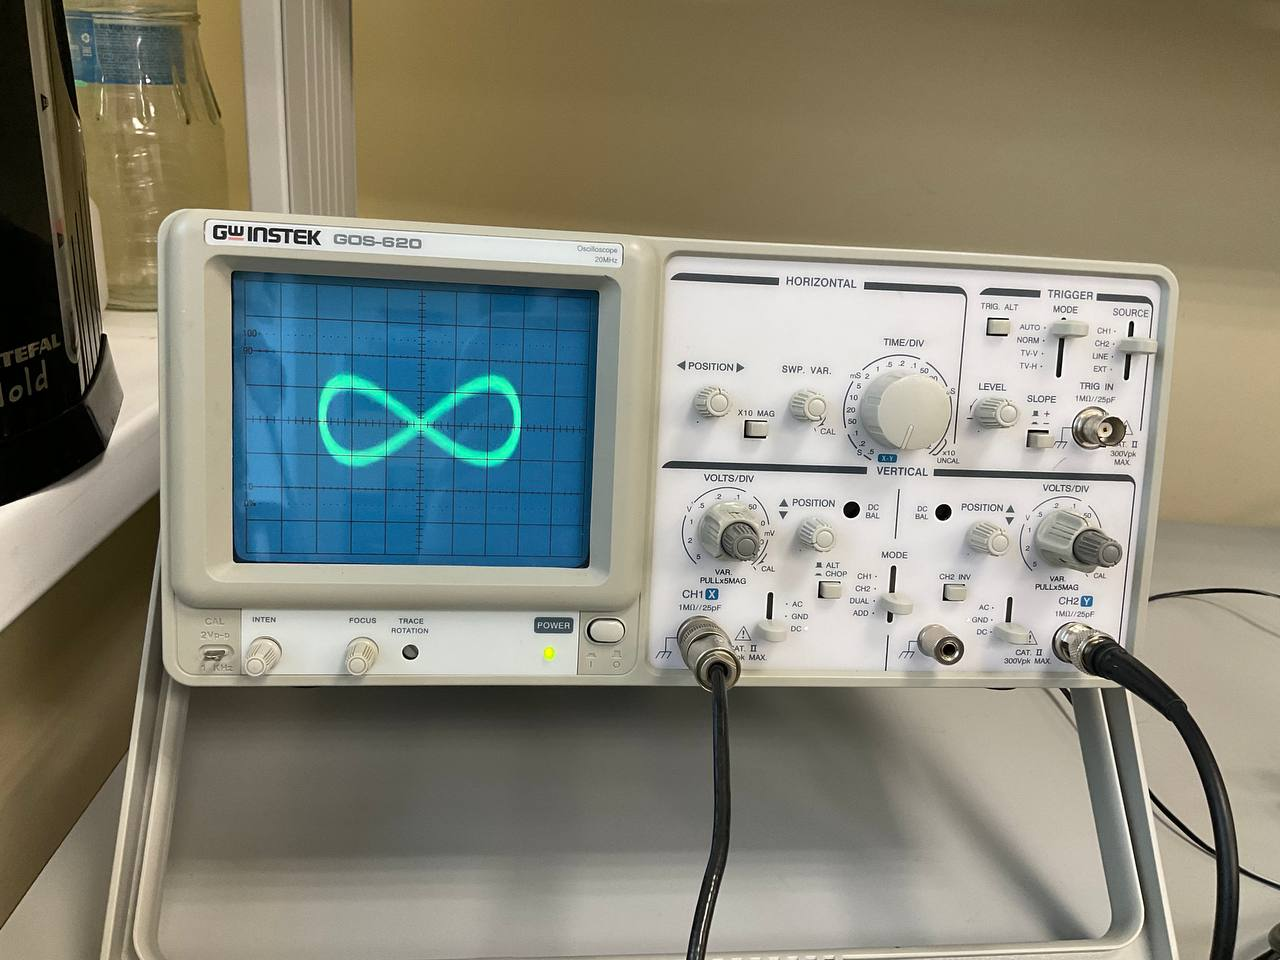
\includegraphics[scale=0.3]{l}
			\caption{Фигура Лиссажу}
			\label{pic4}
		\end{figure}

		\item Не выполнялся.
		\item Не выполнялся.
		\item Построим графики зависимости частоты от номера гармоники $f(n)$ для каждого стержня.
		\begin{figure}[h!]
			\centering
			\begin{tikzpicture}[dot/.style = {draw, fill = black, color = black, circle, inner sep=1.5pt}, >=stealth]
				\begin{axis}
					[
					width = 0.68\paperwidth, 
					xlabel = {$n$}, 
					ylabel = {$f$, Гц},
					%grid=both, 
					ymin = 0, %ymax = 0.2,
					xmin = 0, %xmax = 70,
					xtick={1,2,...,5},
					%ytick={0.1,0.15,0.2},
					]
					
					\addplot+[black,only marks,mark = *,
					mark options = {
						scale = 1.0, 
						fill = black
					}] coordinates {(1, 3248.7) (2, 6501.0) (3, 9726.0) (4, 12979.3) (5, 16232.0)};
					\addplot+[green,only marks,mark = *,
					mark options = {
						scale = 1.0, 
						fill = black
					}] coordinates {(1, 4129.3) (2, 8273.0) (3, 12403.7) (4, 16537.3) (5, 20670.3)};
					\addplot+[red,only marks,mark = *,
					mark options = {
						scale = 1.0, 
						fill = black
					}] coordinates {(1, 4256.0) (2, 8549.7) (3, 12777.3) (4, 17033.3) (5, 21273.3)};
					\addplot[black, domain=0:5.5] {3244.5 * x + 3.9};
					\addplot[green, domain=0:5.5] {4134.6 * x - 1.2};
					\addplot[red, domain=0:5.5] {4251.8 * x + 21.5};
				\end{axis}
			\end{tikzpicture}
			\caption{График зависимости $f$ от $n$}
			\label{graph1}
		\end{figure}

		На графике черным цветом представлена зависимость для меди, зеленым -- для стали, красным -- для алюминия.
		
		Как видно, зависимость является линейной и проходит через начало координат, что согласуется с теорией.

		\item Построим наилучшие прямые по экспериментальным точкам. Определим коэффициент наклона по формуле
		$$
		k = \frac{\langle x y \rangle - \langle x \rangle \langle y \rangle}{\langle x^2 \rangle - {\langle x \rangle} ^2}
		$$
		Занесем рассчитанные значения в таблицу \ref{table4}.
		\begin{table}[h]
			\centering
			\begin{tabular}{|c|c|c|c|} \hline
				материал & $k$, Гц & $\sigma_k$, Гц & $u$, м/с \\ \hline
				медь & $3244.5$ & $3.7$ & $3893.4 \pm 4.4$ \\ \hline
				сталь & $4134.6$ & $10.0$ & $4961.5 \pm 12.0$ \\ \hline
				алюминий & $4251.8$ & $9.4$ & $5102.2 \pm 11.3$ \\ \hline
			\end{tabular}
			\caption{Коэффициенты наклона}
			\label{table4}
		\end{table}

		Погрешность коэффициента $k$:
		$$
		{\sigma_k}^{\text{сл}}= \sqrt{\frac{1}{n-2}\left(\frac{D_{yy}}{D_{xx}} - k^2 \right)}
		$$
		Величины погрешностей также заносим в таблицу \ref{table4}.

		Скорости звука считаем по формуле 
		$$
		u = 2Lk,
		$$
		где $L = 60$ см, и также записываем в таблицу.

		\item Определим модуль Юнга для каждого стержня по формуле
		$$
		E = u^2\cdot\rho
		$$
		Погрешность величины:
		$$
		\sigma_{E} = \sqrt{\left(\frac{\partial{E}}{\partial{u}}\right)^2\cdot\sigma_u^2 + \left(\frac{\partial{E}}{\partial{\rho}}\right)^2\cdot \sigma_{\rho}^2} = \sqrt{(2u\rho)^2\cdot \sigma_u^2 + u^4\cdot \sigma_{\rho}^2}
		$$
		\begin{table}[h]
			\centering
			\begin{tabular}{|c|c|c|} \hline
				материал & $E$, ГПа & $\sigma_E$, ГПа \\ \hline
				медь & $135.5$ & $0.3$ \\ \hline
				сталь & $193.2$ & $0.9$ \\ \hline
				алюминий & $71.8$ & $0.3$ \\ \hline
			\end{tabular}
			\caption{Модули Юнга}
			\label{table4}
		\end{table}
		Результаты совпадают с табличными данными.

		\item Не выполнялся.
	\end{enumerate}
\subsection*{Вывод}
В результате эксперимента получили значения скорости звука в представленных материалах и модули Юнга этих материалов.	
Достижение такой хорошей точности возможно благодаря высокой чувствительности генератора колебаний. Однако достаточно большую погрешность в результаты измерений вносит неточность определения резонанса визуальным методом, так как не всегда каринка на осциллографе получалась чёткой и отличалась при изменении частоты колебаний.	

\end{document}
